%\documentclass[../main.tex]{subfiles}


\begin{song}{title=\centering Je jaká je \\\normalsize Karel Gott  \vspace*{-0.3cm}}  %% sem se napíše jméno songu a autor
\moveright 2cm \vbox{      %Varianta č. 1  ---> Jeden sloupec zarovnaný na střed

\sloka
Je,^{D} jaká ^{F#mi G}je, tak mi ^{A{\color{white}\_\_}}náhle padla ^{D}do ^{{\color{white}\_\_\_}F#mi}klína, 

^{G}ani ^{A{\color{white}\_\_}}černá ani ^{{\color{white}\_\_\_}D\,\,{\color{white}\_\_}F#mi G}blondýna, někdy ^{A}tak a jindy ^{D{\color{white}\_\_}}taková, ^{Hmi}

^{G}vždycky ^{A{\color{white}\_\_}}hádám. jak se ^{{\color{white}\_\_\_}D{\color{white}\_\_}Hmi G}zachová, zřejmě ^{A{\color{white}\_\_}}nikdy, jak chci ^{D}já. ^{Hmi G A}

\sloka
Je, jaká je -- trochu dítě, trochu mondéna, 

nemám právě paměť na jména, tak jí říkám lásko má. 

Nejsi skvost a nejsi zlá, jsi jen jiná, než chci já. 

\sloka
Je, jaká je, že se změní čekat nedá se, 

snad jí záleží jen na kráse, tak, že člověk málem nedutá, 

jak je štíhlá, jak je klenutá, jenže jinak, než chci já. 

\sloka
Je, jaká je, až jí zitra spatříš u pláže, 

vzkaž jí, ať se na mě neváže, ať si pro mě vrásky nedělá, 

ať je jaká je a veselá, i když jiná, než chci já. 
}
\setcounter{Slokočet}{0}
\end{song}


\begin{figure}[h]
\centering
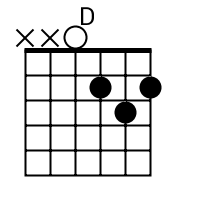
\includegraphics[width=3cm]{../Akordy/d.png}
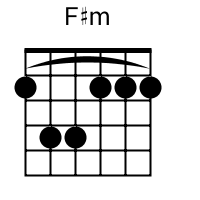
\includegraphics[width=3cm]{../Akordy/fxm.png}
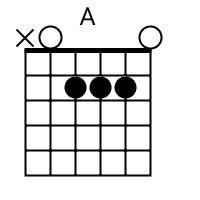
\includegraphics[width=3cm]{../Akordy/a.png}
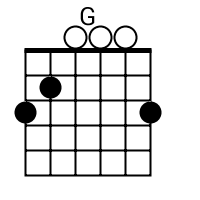
\includegraphics[width=3cm]{../Akordy/g.png}
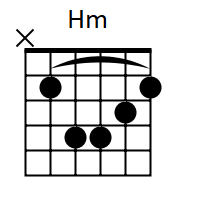
\includegraphics[width=3cm]{../Akordy/hm.png}
\end{figure}

